El objetivo de este proyecto es generar un lazo de control que tenga como entrada la velocidad de referencia, y que contemple las perturbaciones externas del sistema en el cálculo de la velocidad de salida que se utilizará como lazo de realimentación (Figura \ref{fig:diagr}). 
Para esto es necesario adaptar la acción de control que se será la entrada de referencia para indicar la frecuencia de salida del variador de velocidad.
Además se espera realizar una interfaz gráfica para un mejor manejo y control del sistema.

\begin{figure}[htb]
	\centering
	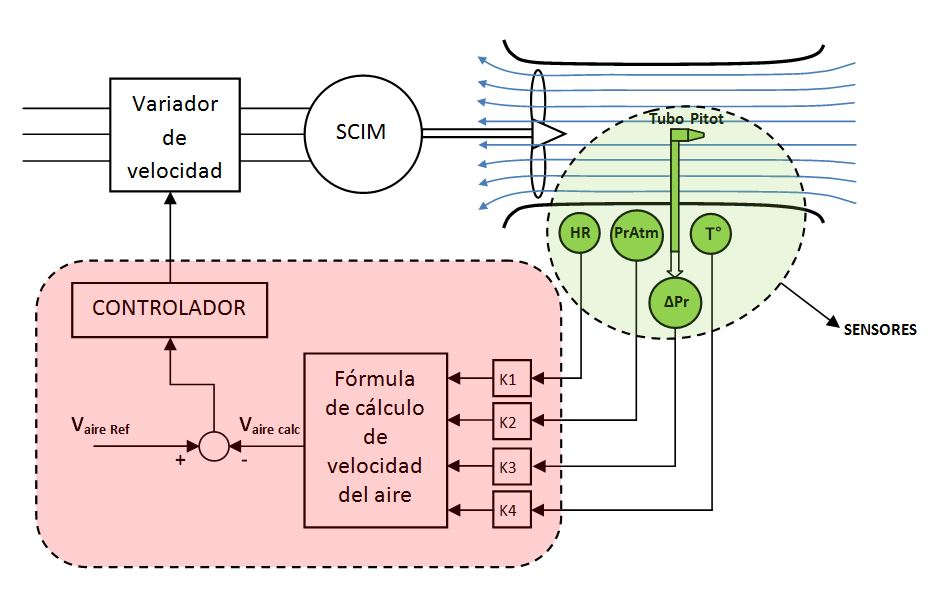
\includegraphics[scale=0.5]{diagr.jpg}
	\caption{Diagrama del objetivo}
	\label{fig:diagr}
	\end{figure}


	\newpage